\section{Versuch 3 - Auswertung der Motorgeschwindigkeit}
Der Motortreiber liefert ein analoges Spannungssignal, welches die aktuelle Motorgeschwindigkeit wiedergibt. Um die ADC-Werte in SI-Einheiten wird ein Polynom erster Ordnung benötigt. Hierfür werden mit Hilfe der ESCON-Studio konstante Motorgeschwindigkeiten ($\dot{\psi} \in \{ -3000, -2000,$  $-1000, 0, 1000, 2000, 3000 \} [rpm] $) gefahren und pro Durchlauf $m=500$ ADC-Werte aufgenommen. Über die Mittelwerte der Messungen und die vorgegebenen Radgeschwindigkeiten wird anschließend ein Polynom erster Ordnung approximiert.

\begin{figure}[h]
	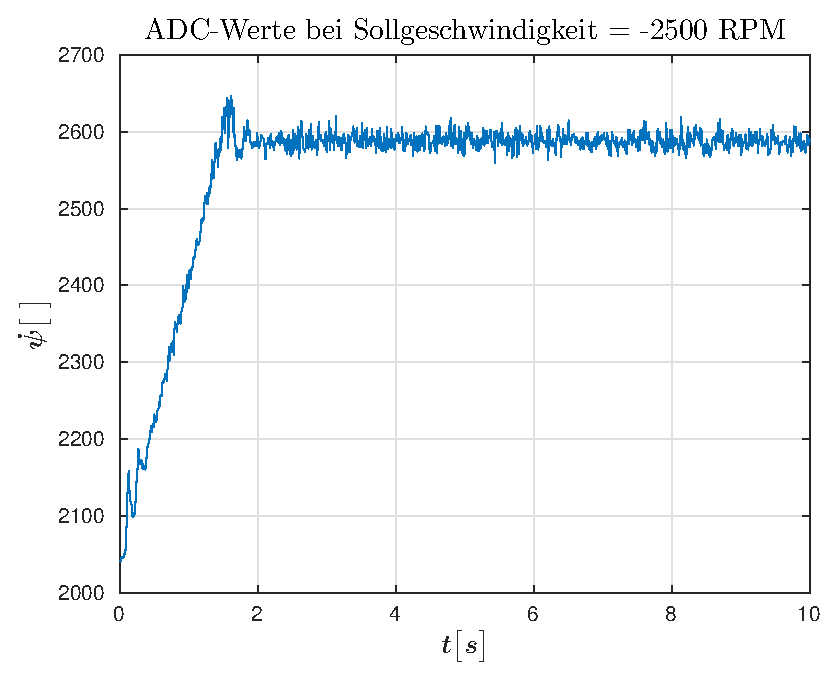
\includegraphics[width=0.5\linewidth]{img/psi1__d___rpm_-2500.eps}
	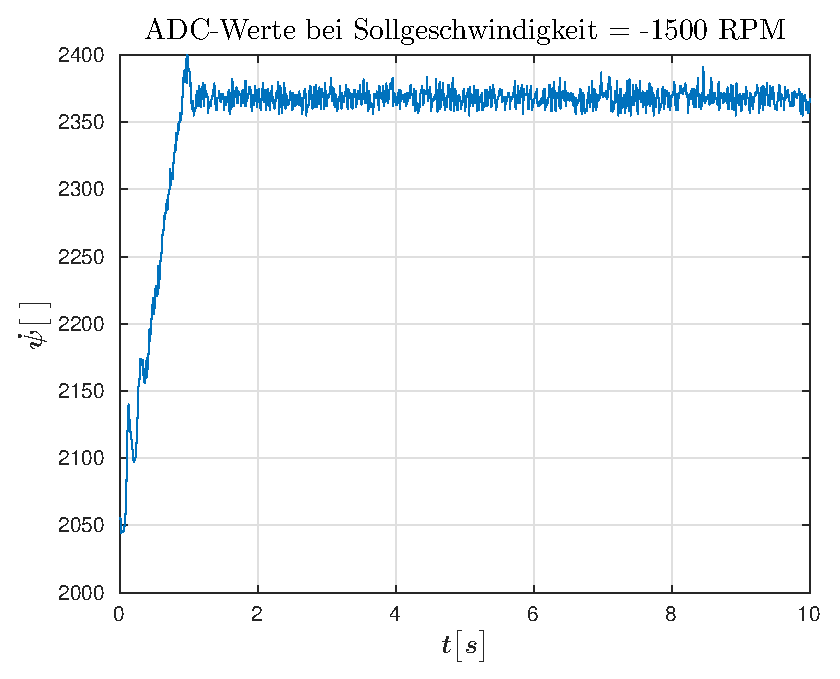
\includegraphics[width=0.5\linewidth]{img/psi1__d___rpm_-1500.eps}
\end{figure}
\begin{figure}[h]
	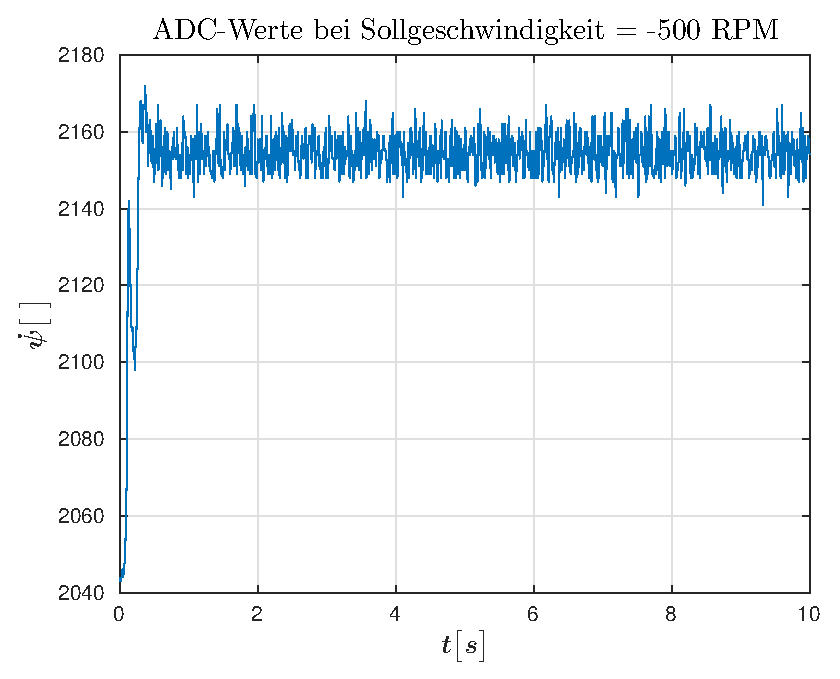
\includegraphics[width=0.5\linewidth]{img/psi1__d___rpm_-500.eps}
	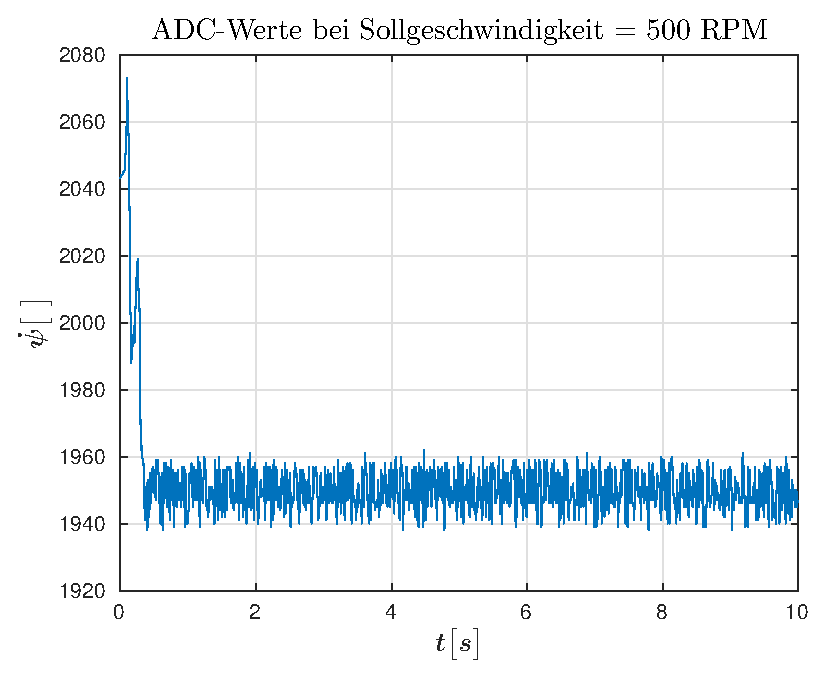
\includegraphics[width=0.5\linewidth]{img/psi1__d___rpm_500.eps}
\end{figure}

\newpage
\begin{figure}[h]
	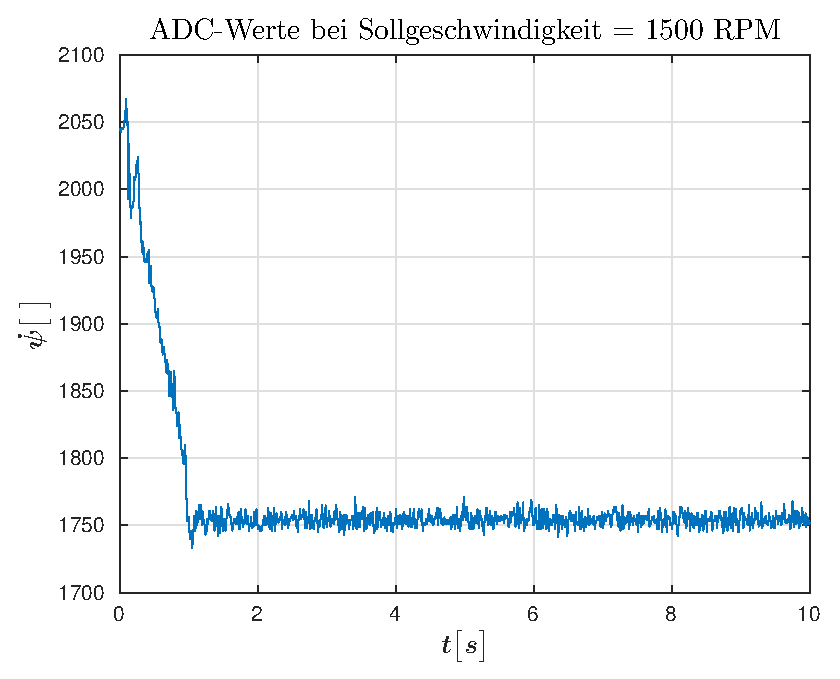
\includegraphics[width=0.5\linewidth]{img/psi1__d___rpm_1500.eps}
	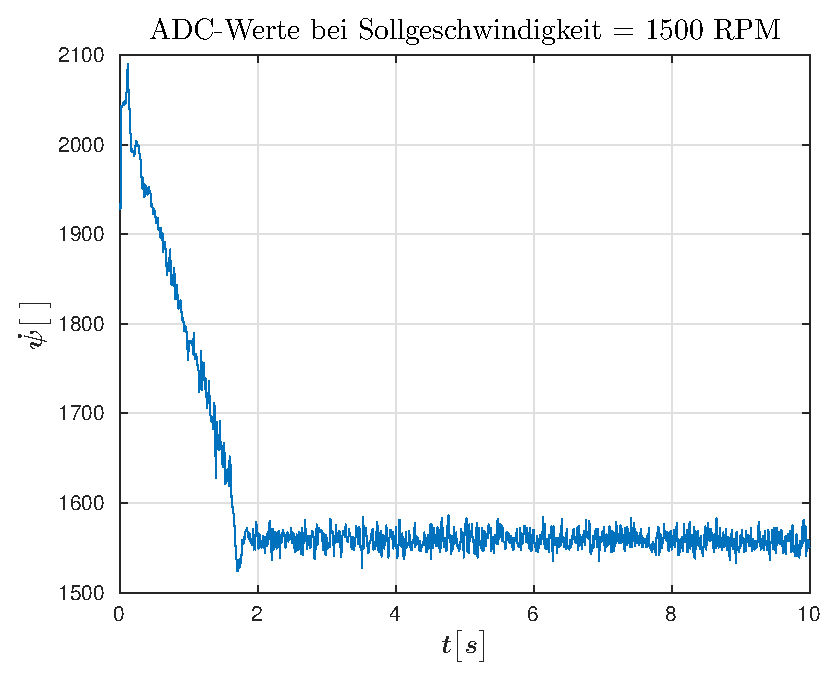
\includegraphics[width=0.5\linewidth]{img/psi1__d___rpm_2500.eps}
\end{figure}

Mit Hilfe von MATLAB  wird ein Polynom erster Ordnung bestimmt, welches die ADC-Werte in SI-Einheiten umrechnet.

\begin{table}[h!]
\centering
\begin{tabular}{lcllcl}
$\dot{\psi}$ & $\equiv$ & Geschwindigkeit der Schwungmasse & $\dot{\psi}_{ADC}$ & $\equiv$ & ADC-Wert
\end{tabular}
\end{table}

\begin{equation}
\dot{\psi} = -0.5092 \cdot \dot{\psi}_{ADC} + 1050
\end{equation}

\begin{figure}[h!]
\centering
	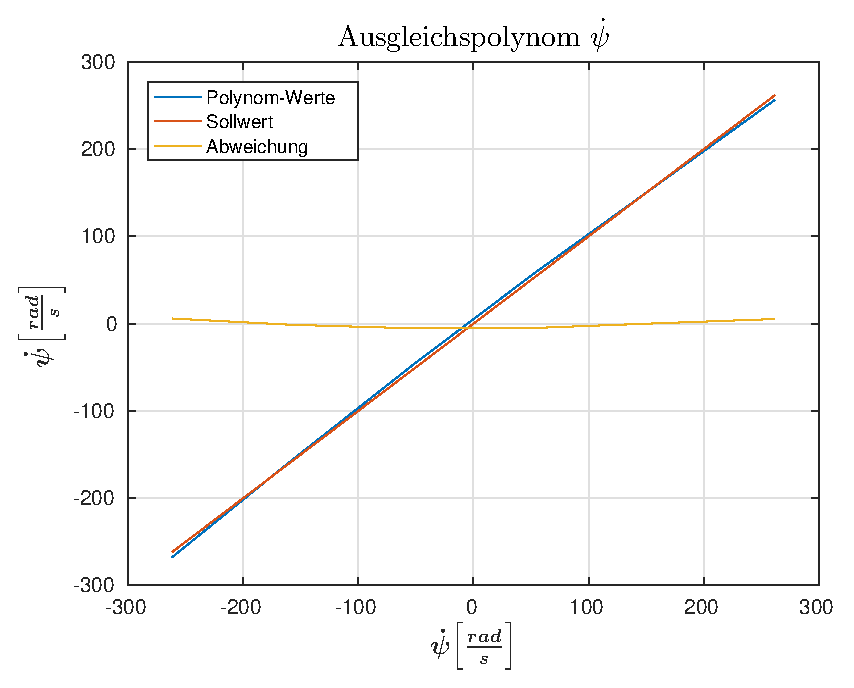
\includegraphics[width=0.5\linewidth]{img/ADC_mittelwert_polynom.eps}
\end{figure}